\section{Can LLMs help identify \emph{When and Which} agent causes task failures?}

As revealed in Section~\ref{sec:dataset_analysis}, detecting the failure-responsible agent and corresponding failure step in agentic system are often subtle, requiring significant human effort. 
Given these challenges, we were thinking of performing automated failure attribution, using LLMs themselves to detect these errors and provide signal for human to perform essential improvement. 
In this section, we set up experiments to answer a fundamental question: 
\textit{Can LLMs help identify \emph{when and which} agent causes task failures in multi-agent systems?} 

\subsection{LLMs for Failure Attribution in Agentic Systems}

To answer the question mentioned above, we propose three judgement methods for automated failure attribution in agentic systems.
Through extensive experiments, we demonstrate that each method has distinct advantages and limitations, and they can be applied either independently or in combination. 
Furthermore, we analyze the performance of these methods across various scenarios and constraints, highlighting their applicability in different contexts.

\textbf{(1) All-at-once:} 
An LLM is provided with a query and the complete failure log, and it is tasked with identifying the failure-responsible agent as well as the specific step where the decisive error occurred. 
\textbf{(2) Step-by-step:}
An LLM is provided with a query, and the failure log is presented step-by-step. At each step, the LLM is tasked with determining whether a mistake has occurred in the current step. If a mistake is identified, the judging process terminates, and the responsible agent's name along with the current step number are returned as the output. Otherwise, the process continues until the final step is reached. 
\textbf{(3) Binary search:}
Alternatively, this method uses a receptive field approach that lies between the previous two methods. Starting with the query and the full failure log, the LLM is tasked with determining whether the mistake occurred in the upper half or lower half of the failure logs. Once this decision is made, the LLM is provided with the selected half of the log and the process is repeated iteratively until a single step is identified. 
The three algorithms and corresponding prompts are detailed in Appendix~\ref{app:algorithm_details} and Appendix~\ref{section:prompt}.


\begin{table*}[!t]
\centering
\renewcommand{\arraystretch}{0.99}
\scalebox{0.99}{
\begin{tabular}{cccccc}
\toprule[1.5pt]
\multicolumn{1}{c|}{}                                   & \multicolumn{2}{c|}{\textbf{With Ground Truth}}                                           & \multicolumn{2}{c}{\textbf{Without Ground Truth}}                                           \\ \cline{1-5}
\multicolumn{1}{c|}{\textbf{Agentic Systems Types}}                                   & \multicolumn{1}{c}{Algorithm Generated} & Hand Crafted & \multicolumn{1}{c}{Algorithm Generated} & Hand Crafted \\\hline
\rowcolor{gray!50} \multicolumn{5}{c}{Random}                                                                                                                                                                                                          \\\hline
\multicolumn{1}{c|}{Agent-Level Accuracy}             & \multicolumn{1}{c}{\cellcolor{gray!0}   29.10} & \cellcolor{gray!0}   
 12.00  & \multicolumn{1}{c}{\cellcolor{gray!0}  29.10} & \cellcolor{gray!0}  12.00                        \\
\multicolumn{1}{c|}{Step-Level Accuracy}                & \multicolumn{1}{c}{19.06} & 4.16    & \multicolumn{1}{c}{19.06} & 4.16                   \\
\rowcolor{gray!50} \multicolumn{5}{c}{All-at-Once}                                                                                                                                                                                                          \\\hline
\multicolumn{1}{c|}{Agent-Level Accuracy}             & \multicolumn{1}{c}{\cellcolor{gray!0}   \textbf{54.33}} & \cellcolor{gray!0}   
 \textbf{55.17}  & \multicolumn{1}{c}{\cellcolor{gray!0}  \textbf{51.12}} & \cellcolor{gray!0}  \textbf{53.44}                        \\
\multicolumn{1}{c|}{Step-Level Accuracy}                & \multicolumn{1}{c}{12.50} & 5.26    & \multicolumn{1}{c}{13.53} & 3.51                   \\
\hline
\rowcolor{gray!50}  \multicolumn{5}{c}{Step-by-Step}                                                                                                                                                                                                         \\\hline
\multicolumn{1}{c|}{Agent-Level Accuracy}               & \multicolumn{1}{c}{35.20} & 34.48  & \multicolumn{1}{c}{26.02} & 32.75                 \\
\multicolumn{1}{c|}{Step-Level Accuracy}                & \multicolumn{1}{c}{\cellcolor{gray!0}  \textbf{25.51}} & \cellcolor{gray!0}  \textbf{7.02}    & \multicolumn{1}{c}{15.31} & \cellcolor{gray!0}  \textbf{8.77}                  \\
\hline
\rowcolor{gray!50}  \multicolumn{5}{c}{Binary Search}                                                                                                                                                                                                         \\\hline
\multicolumn{1}{c|}{Agent-Level Accuracy}               & \multicolumn{1}{c}{44.13} & 51.72   & \multicolumn{1}{c}{30.11} & 36.21                \\
\multicolumn{1}{c|}{Step-Level Accuracy}                & \multicolumn{1}{c}{23.98} & 6.90     & \multicolumn{1}{c}{\cellcolor{gray!0}  \textbf{16.59}} & 6.90                  \\
\bottomrule[1.5pt]
\end{tabular}
}
\caption{Performance of the three failure attribution methods on the Who\&When dataset with and without labels, evaluated on the \texttt{GPT-4o} model. 
For agent-level accuracy, all-at-once outperforms binary search, which in turn surpasses step-by-step. 
Conversely, for step-level accuracy, step-by-step achieves the best performance, followed by binary search and then all-at-once.}
\label{tab:main_results}
\end{table*}

\subsection{Settings}

\paragraph{Scenario.} 
We conduct experiments under two distinct settings to simulate various realistic scenarios.
\textbf{(1) With Ground Truth:} 
In this setting, the final ground truth of the query that the agentic system is attempting to resolve is available to the LLMs. 
Our focus here is on the typical AI system development cycle, where it is common practice to use a development dataset with ground truth to identify and debug potential errors in experimental systems. 
\textbf{(2) Without Ground Truth:} 
In the second setting, the final ground truth of the query is unavailable. In this scenario, LLMs are employed to perform failure attribution in agentic systems based on their running logs. This capability can also be viewed as a form of self-reflection~\citep{shinn2024reflexion, huang2023large}, which contributes to the improvement of multi-agent systems.
Throughout this paper, unless otherwise specified, all results are reported as the average accuracy across these two scenarios.

\paragraph{Models.} 
The primary experiments are conducted using the \texttt{GPT-4o} model, unless otherwise specified. Additionally, we also incorporate several other models, including both open-source (such as the \texttt{Llama} and \texttt{Qwen} series) and closed-source models (\texttt{GPT} series), to ensure the consistency of the conclusions drawn from the experiments.
Additionally, we employ advanced reasoning models, i.e., OpenAI o1 and DeepSeek R1, to assess the performance of reasoning models on failure attribution tasks. The results of these evaluations are provided in Appendix~\ref{app:reasoning}.



\subsection{Overall Performance}
We first perform experiments to compare the performance of three failure attribution methods on Who\&When dataset with \texttt{GPT-4o} model. 
The results are reported on Table~\ref{tab:main_results}. 
\paragraph{Agent-Level Accuracy Relies on Large Receptive Field.} 

As shown in Table~\ref{tab:main_results}, all-at-once significantly outperforms the other two failure attribution methods in agent-level accuracy. 
Specifically, its agent-level accuracy is 19.13\% and 20.69\% higher than step-by-step when judging with ground truth, and 25.1\% and 20.69\% higher when judging without ground truth, respectively.
The performance of the binary search method falls between these two approaches.

These results can be attributed to the fact that predicting the failure-responsible agent requires the judge LLMs to consider a broader context, including the behaviors of multiple agents. Since all-at-once has access to the entire conversation log when making the final judgment, its prediction of the failure-responsible agent is more accurate. In contrast, the step-by-step method processes the conversation history incrementally, while the final decision can be made with incomplete information, thus resulting in lower performance. 
Moreover, all failure attribution methods outperform the random baseline, highlighting that these approaches are nontrivial and affirming the necessity of involving LLMs for failure attribution.

\finding{1}{Providing broader failure log context enables more accurate agent-level failure attribution by incorporating more complete information.}

\paragraph{Fine-Grained Predictions Boost Better Step-Level Accuracy.}

\begin{figure}[!t]
    \centering
    \subfigure{
        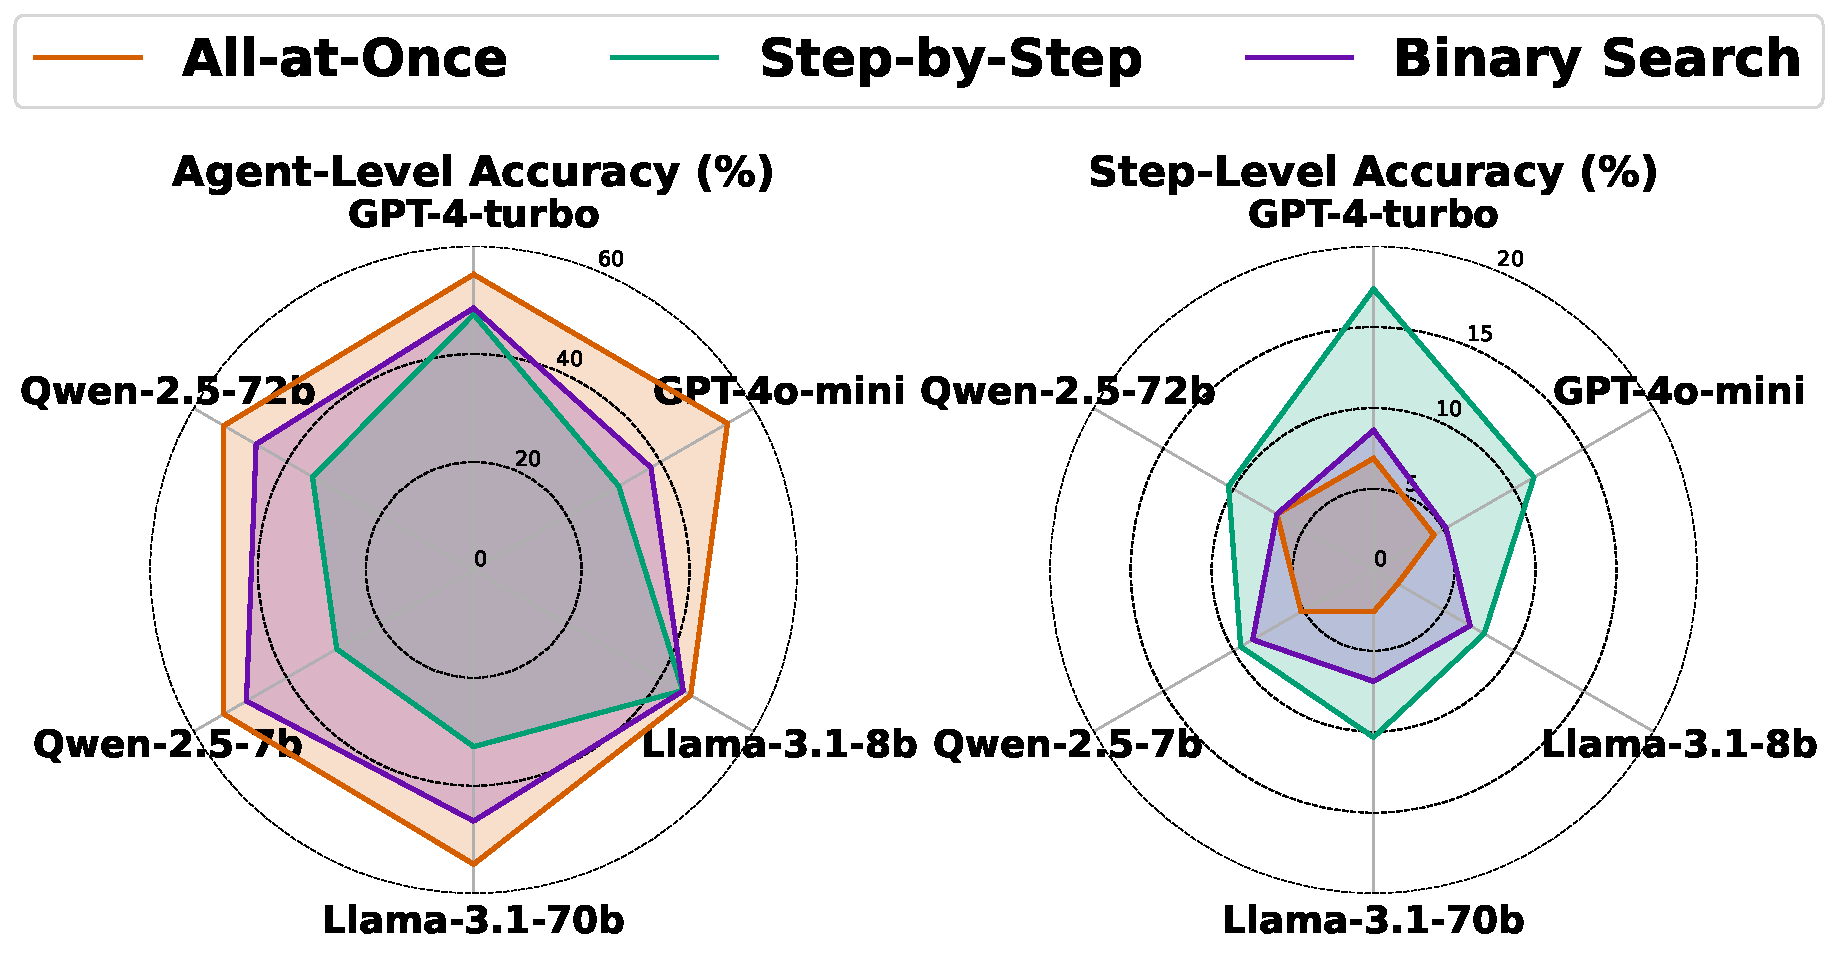
\includegraphics[width=0.49\textwidth]{fig/radar.pdf}
    }
    \caption{Performance comparison of three failure attribution methods on different models in both two metrics. We found the conclusion is mostly consistent with Table~\ref{tab:main_results}.}
    \label{fig:different_model}
\end{figure}


In terms of step-level accuracy, the all-at-once approach performs obviously the worst, even with its average performance falling below that of random method. This outcome underscores the method's practical infeasibility. 
By contrast, the step-by-step approach achieves the highest performance, outperforming other methods in step-level accuracy in 3 out of 4 cases. The performance of the binary search method still falls between these two approaches.

These two results can be attributed to the 'space-in-the-needle' problem, where LLMs often struggle to retrieve specific information from long contexts~\citep{nelson2024needle}.
The all-at-once method has access to the largest context when making decisions about the decisive error step, but this can lead to difficulties in pinpointing the exact failure step within a long history. 
In contrast, the step-by-step method processes the context incrementally, allowing for more focused decision-making. The binary search method performs at a level between these two approaches.

\finding{2}{Incrementally processing context enables better step-level failure attribution since LLMs struggle to retrieve information from long contexts.}

\paragraph{Impact of Ground Truth on Failure Attribution.}
We also observed that failure attribution accuracy is higher for all three methods when ground truth are available, compared to when judgments are made without ground truth in all cases in all metrics.
Although the answers to users' queries may not serve as definitive 'golden labels' for each agent's correct behavior, they provide a useful reference signal for the judgment LLMs. 
For instance, if an agent leads the system in a completely wrong direction, with no possibility of reaching the correct final answer, the label information can directly help alert the judgment LLMs to this error.
Without such intervention, the entire system might proceed in the wrong direction without any external warning. 
\paragraph{Consistency of Conclusions Across Various LLMs.}
In addition to the \texttt{GPT-4o} model, we conducted evaluations on other LLMs, including open-source models (e.g., the Llama series and Qwen series) as well as closed-source models (e.g., the GPT series).
Due to the significant computational and token costs, we only perform experiments on hand-crafted agentic systems from Who\&When which has fewer failure logs. The results of three methods are shown in Figure~\ref{fig:different_model}.
We found that the phenomena observed in Table~\ref{tab:main_results} hold consistently across different LLMs. 
Specifically, for agent-level accuracy, the ranking is: all-at-once, followed by binary search, and then step-by-step. Conversely, for step-level accuracy, the ranking is: step-by-step, followed by binary search, and then all-at-once.

\finding{3}{The pros and cons of different failure attributions methods in this study are mostly consistent across different LLMs.}

\begin{figure}[!t]
    \centering
    \subfigure[Agent-Level Accuracy]{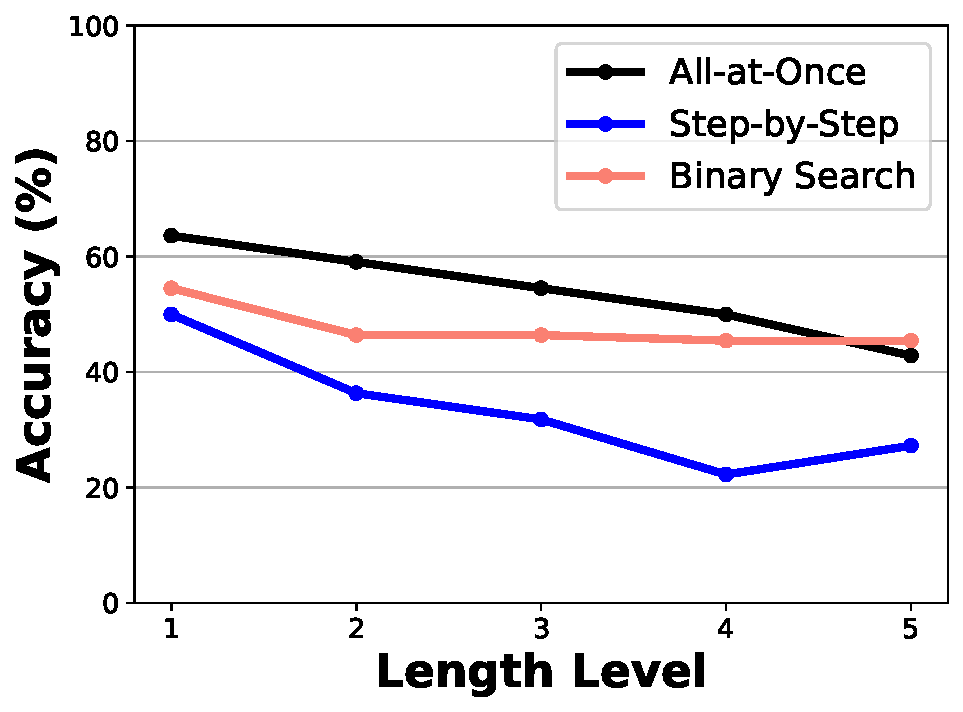
\includegraphics[width=0.238\textwidth]{fig/length_performance_agent_level_acc.pdf}}
    \subfigure[Step-Level Accuracy]{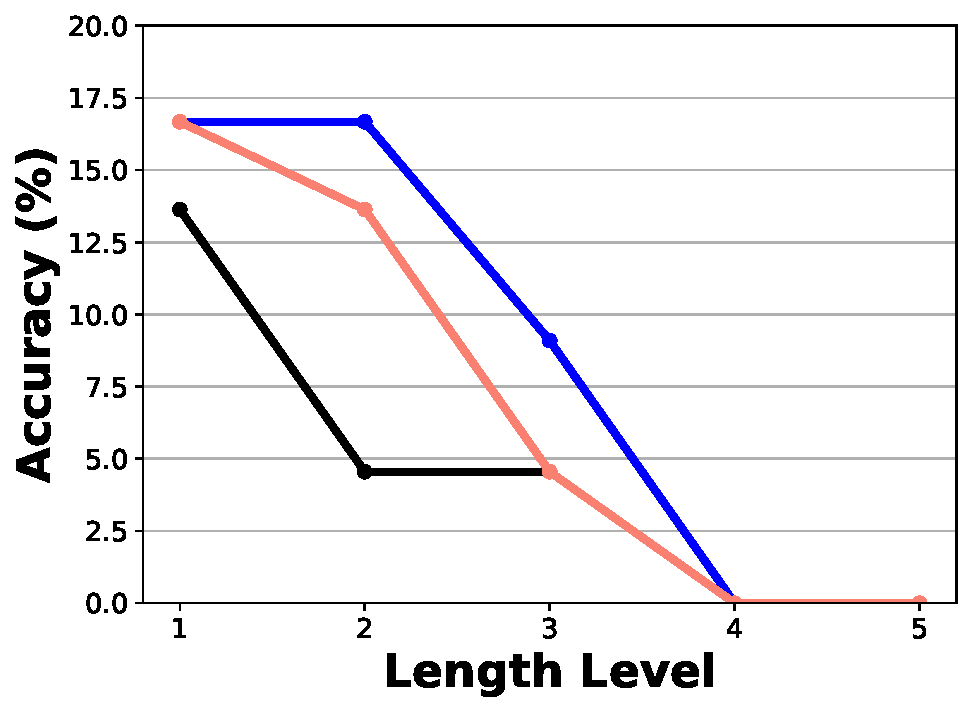
\includegraphics[width=0.235\textwidth]{fig/length_performance_step_level_acc.pdf}}
    \caption{Comparison of three failure attribution methods applied to all failure logs from the hand-crafted systems in the Who\&When, evaluated under varying failure log lengths across both metrics.}
    \label{fig:different_length}
\end{figure}

\subsection{Performance Across Varying Context Lengths}

We investigate the relationship between the length of failure logs and the corresponding failure attribution performance. 
Specifically, the failure logs of hand-crafted agentic systems from the Who\&When dataset are divided into five levels, with context length progressively increasing from Level 1 to Level 5. Specifically, Level 1 spans 5–17 steps, Level 2 covers 19–29, Level 3 includes 31–49, Level 4 ranges from 51–91, and Level 5 spans 93–130 steps.
Both agent-level and step-level judgment performances across the three evaluation methods are presented in Figure~\ref{fig:different_length}. 
Algorithm-generated systems are excluded from this analysis due to their limited maximum step count of 10, which prevents meaningful divisions of context length.

Our findings indicate that all three methods exhibit a decline in both metrics as context length increases. Notably, step-level accuracy is more sensitive to context length changes than agent-level accuracy. Furthermore, the step-by-step performance decline is particularly pronounced compared to the other two.
We also analyze the distances between human-annotated decisive error steps and the predicted steps for each data instance, as shown in Figure~\ref{fig:step_distance}. These results demonstrate that the step-by-step method outperforms the other two methods in accurately predicting the decisive error steps.
However, as context length reaches its maximum, all three failure attribution methods converge to near 0\%, as shown in Figure~\ref{fig:different_length}.
 
\finding{4}{Failure attribution performance declines as context length increases, with step-level accuracy being more sensitive.}

\subsection{Step-Level Accuracy Under Different Tolerances}

\begin{table}[!htb]
\renewcommand{\arraystretch}{0.95} 
\scalebox{0.96}{
\begin{tabular}{llll}
\toprule[1.5pt] \rowcolor{gray!50}
 \textbf{Toler.}   & \textbf{All-at-Once} & \textbf{Step-by-Step} & \textbf{Binary Search} \\ \hline
$\pm$ 1 & 12.07       & \textbf{14.66}        & 13.79         \\
$\pm$ 2 & \textbf{19.83}       & 16.38        & 18.97         \\
$\pm$ 3 & \textbf{30.17}       & 18.10        & 22.41         \\
$\pm$ 4 & \textbf{37.07}       & 31.90        & 31.89         \\
$\pm$ 5 & \textbf{43.10}       & 33.62        & 36.21         \\ \bottomrule[1.5pt]
\end{tabular}}
\caption{Step-level accuracy with different tolerances on the failure logs of hand-crafted agentic systems from Who\&When dataset.}
\label{table:tolerance}
\end{table}

\begin{figure}[!t]
    \centering
    \subfigure[Algorithm-Generated]{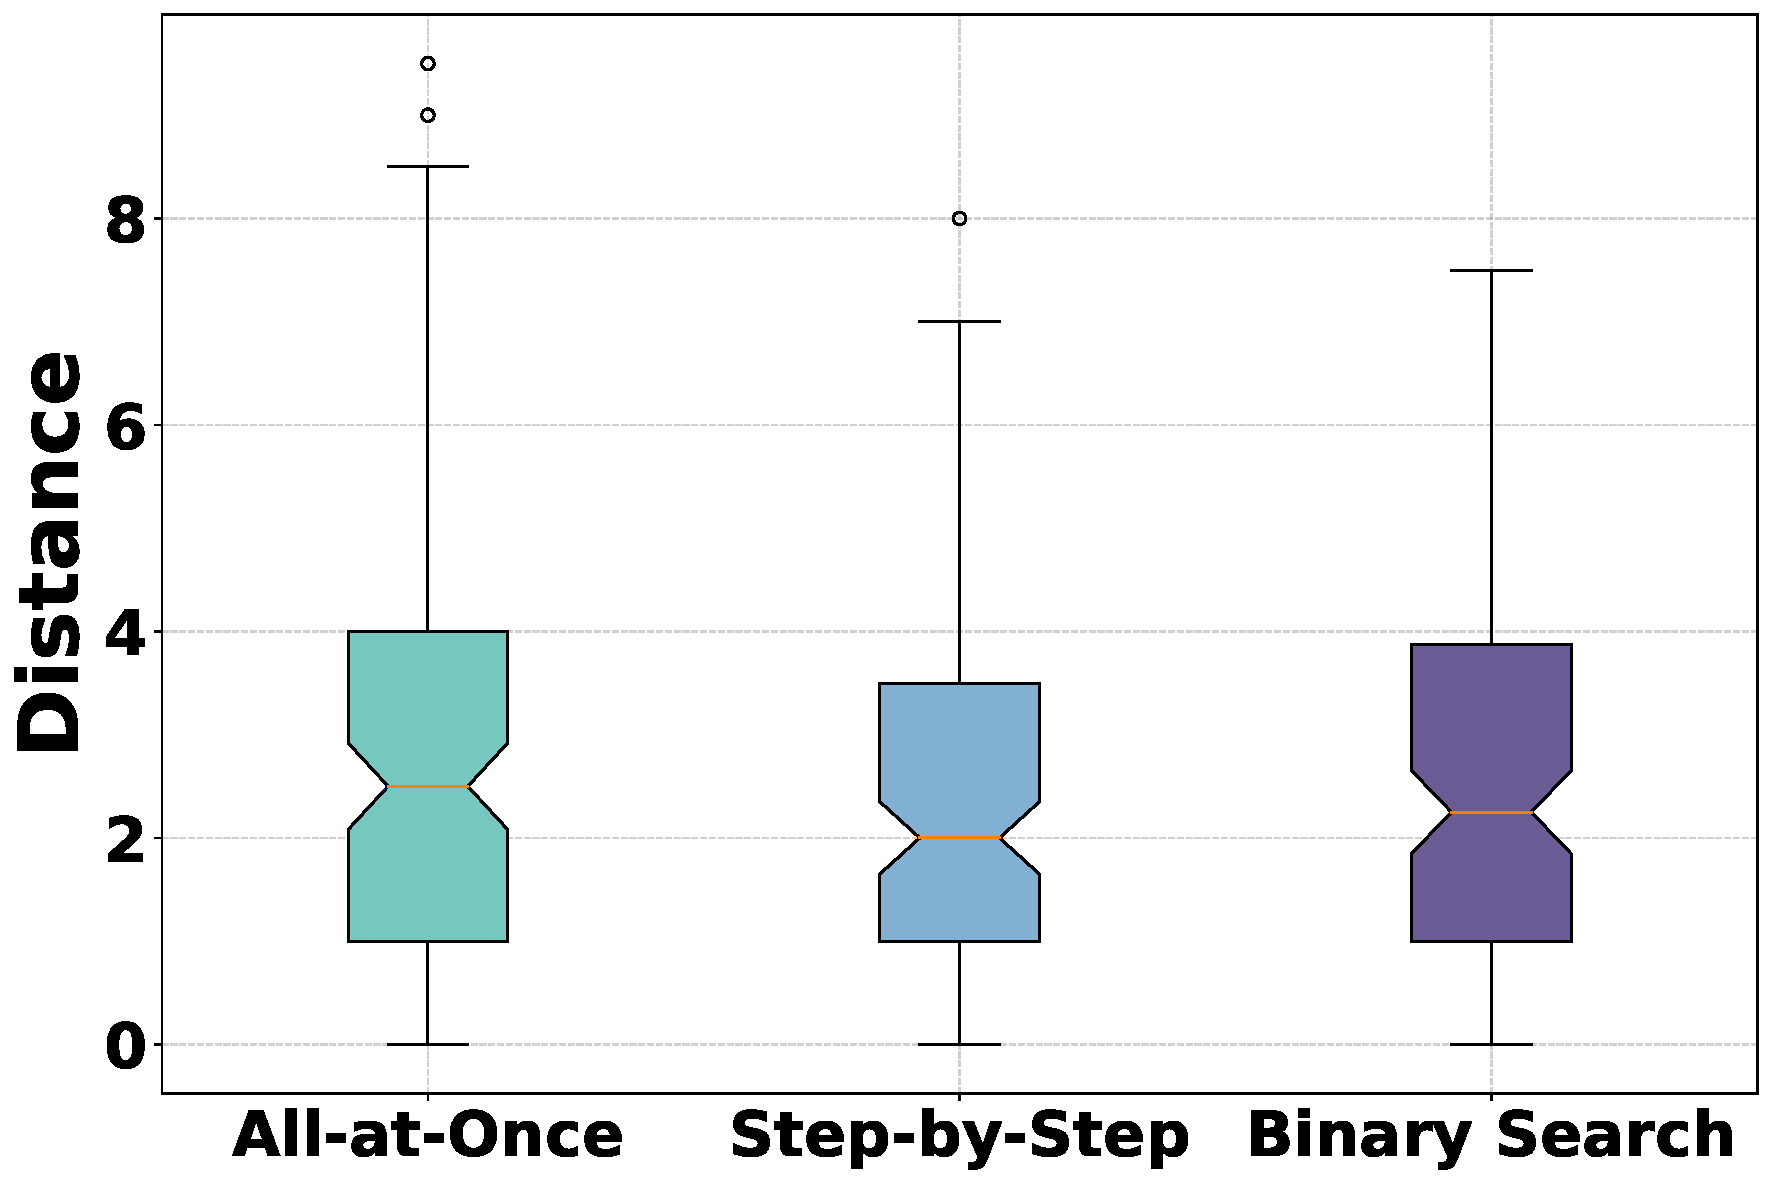
\includegraphics[width=0.235\textwidth]{fig/cap_box.pdf}}
    \subfigure[Hand-Crafted]{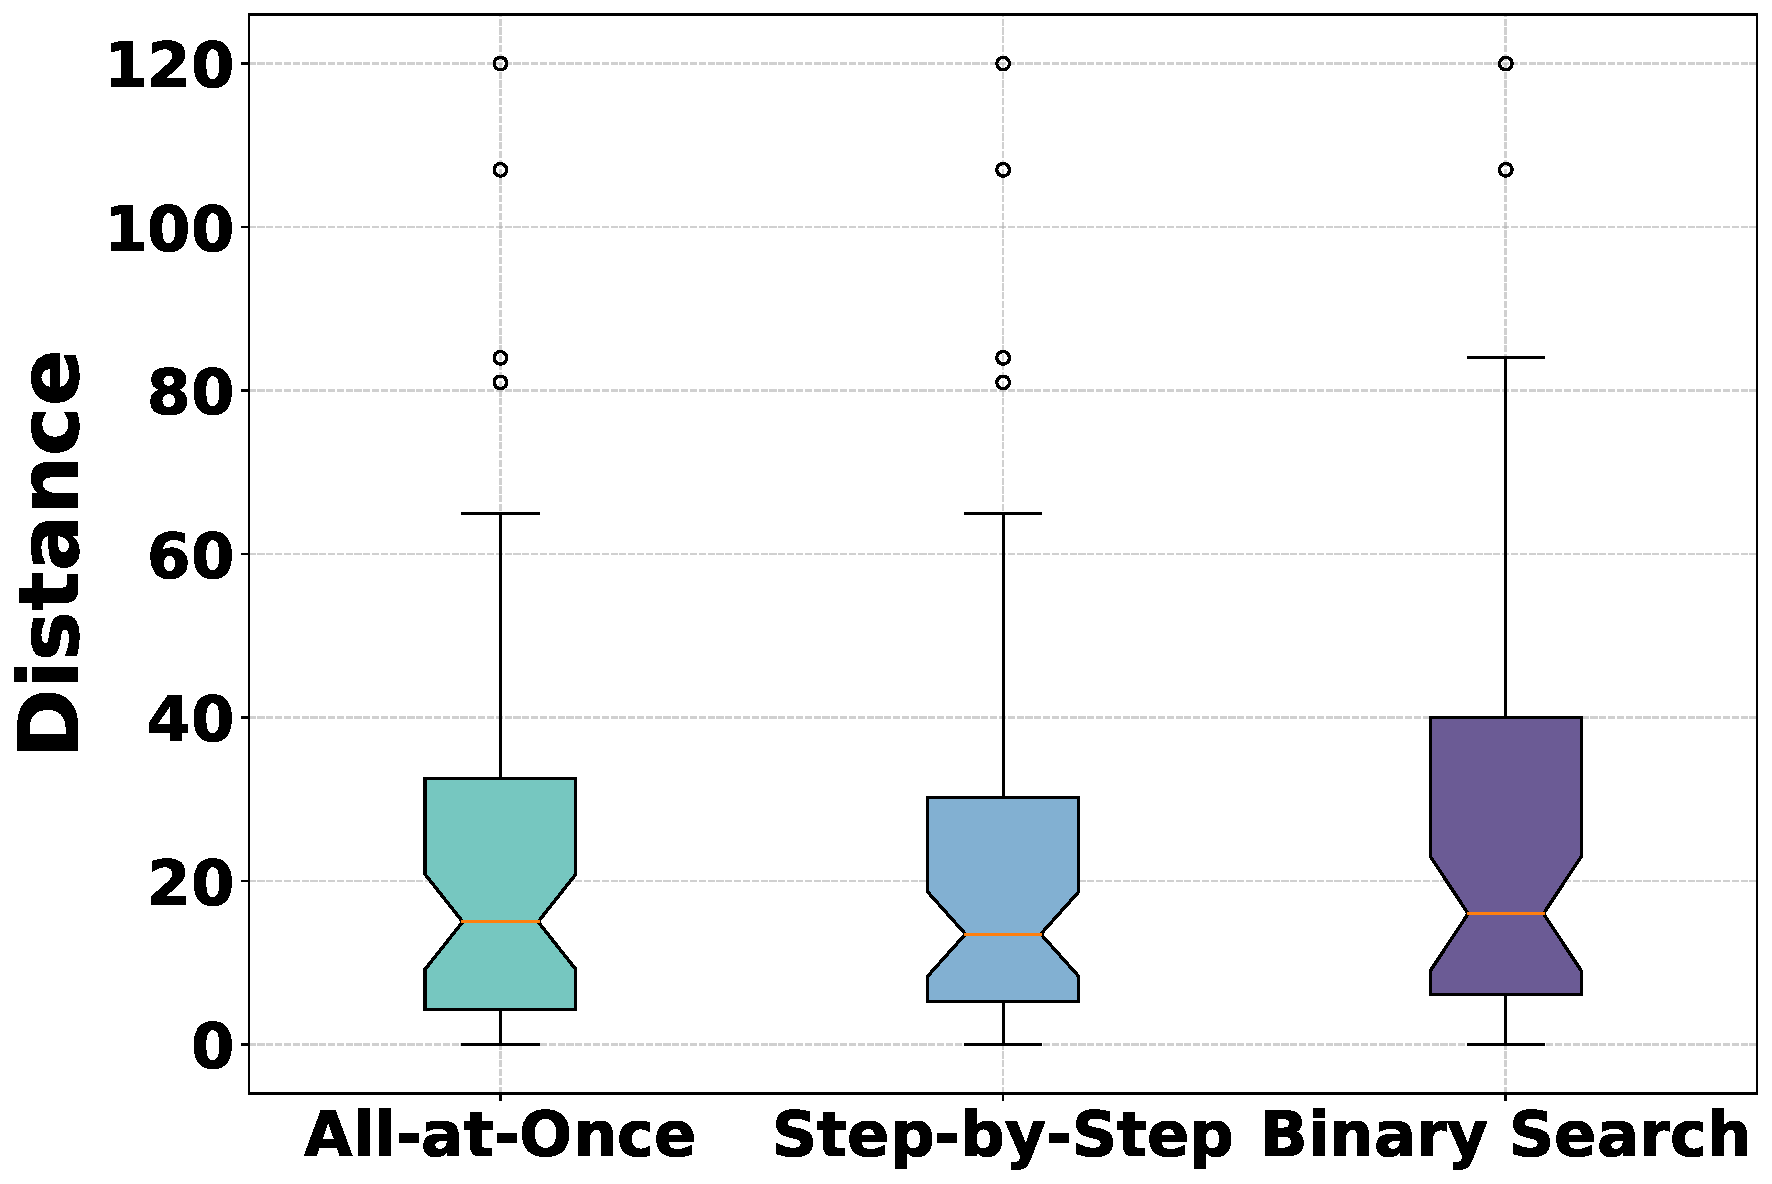
\includegraphics[width=0.235\textwidth]{fig/mag_box.pdf}}
    \caption{The distances between human-annotated decisive error steps and the predicted steps for each date instance on failure logs from both algorithm-generated and hand-crafted systems.}
    \label{fig:step_distance}
\end{figure}



In practice, directly identifying the exact decisive error step is not always necessary; it is often sufficient to determine a range of steps where the mistake might occur. In this section, we show the performance of the three failure attribution methods under varying tolerance conditions on the failure logs of hand-crafted agentic systems from the Who\&When dataset. Algorithm-generated systems are excluded from this analysis because their maximum step count is limited to 10, and increasing the tolerance would lead to artificially inflated accuracy.

As shown in Table~\ref{table:tolerance}, our findings show that step-by-step achieves the highest performance when the tolerance is set to $0$ or $1$. However, as the tolerance increases, the advantages of all-at-once become more pronounced, while the benefits of step-by-step diminish. 
Compared to all-at-once, step-by-step demonstrates better alignment with accurate predictions when high precision is required.


\finding{5}{Allowing tolerance in failure attribution enables broader context processing methods to achieve competitive step-level accuracy.}


\subsection{A Statistical Viewpoint on Failure Attribution}

\begin{figure}[!t]
    \centering
    \subfigure{
        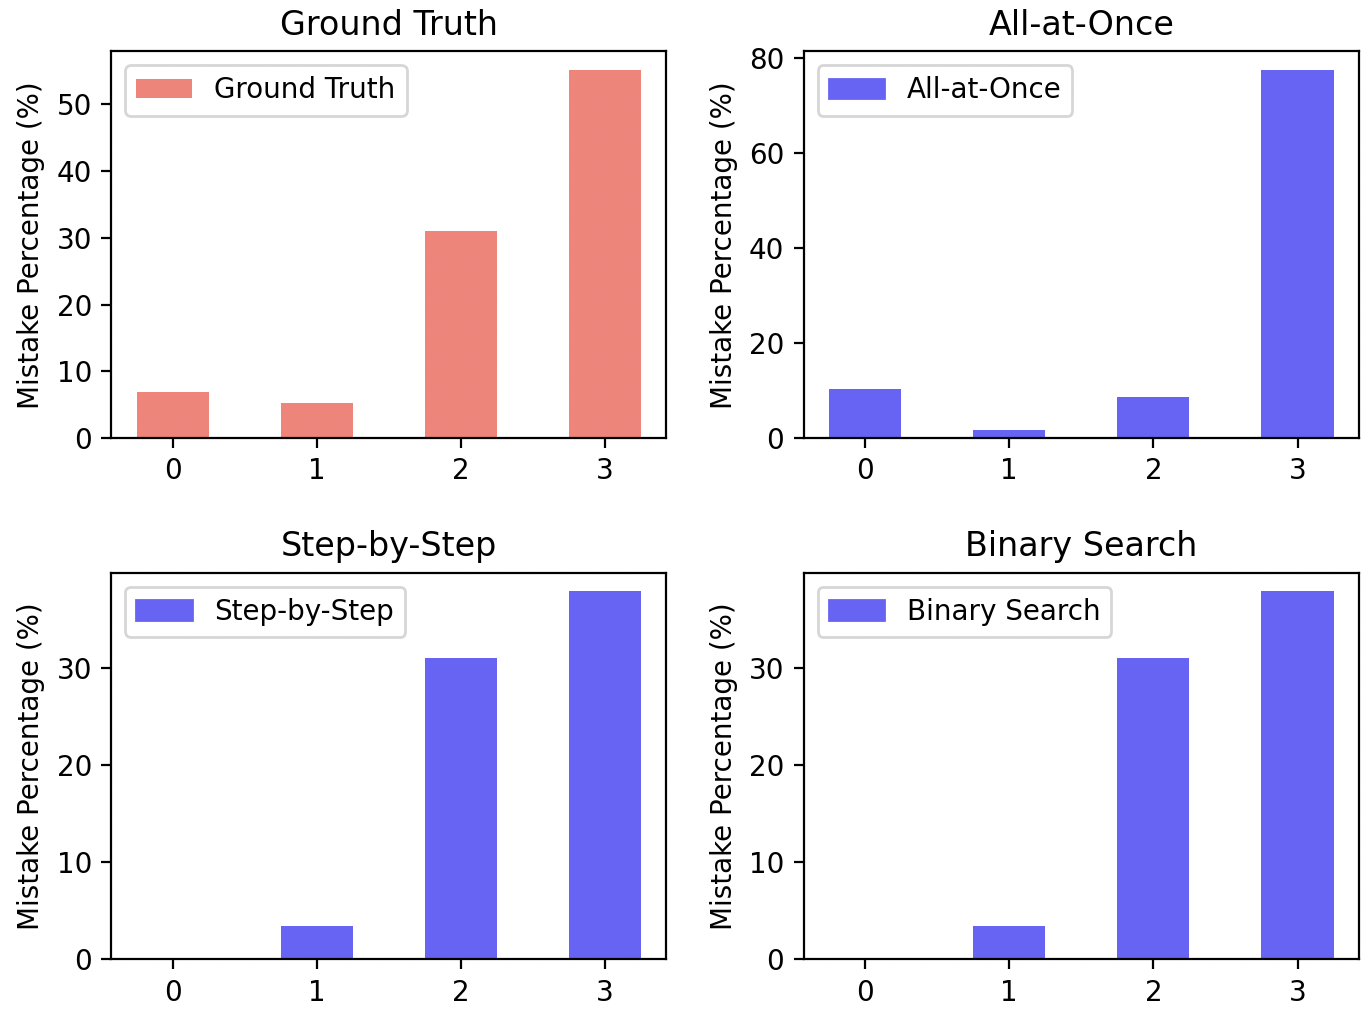
\includegraphics[width=0.47\textwidth]{fig/whole_compare.png}
    }
    \caption{Histogram of the actual and predicted failure-responsible agents for all three methods. We present only the failure logs of hand-crafted systems in Who\&When to aggregate the largest number of results for one multi-agent system. Number 0, 1, 2, 3 represents \texttt{Assistant}, \texttt{FileSurfer}, \texttt{Orchestrator} and \texttt{WebSurfer} respectively.}
    \label{fig:stat_compare}
\end{figure}



This study primarily perform experiments on single-data-level failure attribution in LLM-powered multi-agent systems, i.e., identifying the specific component (referred to as the failure-responsible agent) and the precise location (the decisive error step) responsible for task failure in a single data instance. 
This practice indeed mirrors human procedures for failure attribution and could serves as a foundational tool for deriving statistical-level conclusions. 
Therefore, we think of whether these methods could be applied to entire datasets to extract meaningful statistical results.

In Figure~\ref{fig:stat_compare}, we show the histogram of actual and the predicted failure-responsible agents for all three methods. We only show the failure logs of hand-crafted systems from Who\&When to aggregate the largest number of results for one system type. 
We observe that the single agent that make the most decisive errors predicted by all methods to are consistent with the ground truth (agent 3). 
Moreover, the top two failure-responsible agents predicted by three methods are also consistent with the ground truth in most cases (2 out of 3).
These experiments demonstrate that, although the instance-level failure attribution results are not highly positive, all three methods still yield meaningful insights from a statistical perspective. In practice, these statistical results provide a more actionable basis for system refinement compared to focusing solely on single data instances.

\finding{6}{The three baseline methods are more effective at performing failure attribution at a statistical level than at an instance level.}

\subsection{Can We Combine Multiple Failure Attribution Methods?}

\begin{table}[!htb]
\setlength{\tabcolsep}{1.2 pt} % Reduce column spacing
\scalebox{0.9}{
\begin{tabular}{cccc}
\toprule[1.5pt]
\rowcolor{gray!50}
\textbf{Metrics} & 
\textbf{\begin{tabular}[c]{@{}c@{}}Cost\\Token Num\end{tabular}} & 
\textbf{\begin{tabular}[c]{@{}c@{}}Agent-Level\\ Accuracy\end{tabular}} & 
\textbf{\begin{tabular}[c]{@{}c@{}}Step-Level\\ Accuracy\end{tabular}} 
\\ 
\midrule
Binary Search              & 34,659     & 43.97 & 6.90 \\
$\vartriangle$ All-at-Once & \textbf{17,106}     & \textbf{57.02} & 4.39 \\
$\square$ Step-by-Step     & 87,720     & 35.96 & 7.90 \\
Hybrid Method ($\square$\&$\vartriangle$) & 149,177 & \textbf{57.02} & \textbf{12.28} \\
\bottomrule[1.5pt]
\end{tabular}}
\caption{Comparison of the three failure attribution methods with a hybrid approach that combines all-at-once and step-by-step on the failure logs of hand-crafted systems from the Who\&When dataset. The hybrid method achieves the highest performance in both two metrics but incurs the highest token costs.}
\label{tab:hybrid}
\end{table}

We then investigate whether a hybrid method could leverage the advantages of both two different methods, all-at-once and step-by-step. The former excels at failure-responsible agent predictions, while the latter is better at accurately predicting the decisive error step.
Specifically, we start by prompting all-at-once to predict the failure-responsible agent and then use step-by-step to detect the mistake step in the actions step taken by the identified failure-responsible agent. 
To evaluate this, we perform experiments on the hand-crafted systems from the Who\&When dataset considering the token cost.  The results are shown on Table~\ref{tab:hybrid}.

We observe that the hybrid method outperforms all methods in step-level accuracy.
This improvement is attributed to the all-at-once narrowing the range of possible failure steps by excluding action steps taken by other agents, thereby significantly reducing the difficulty of prediction for step-by-step. 
However, the hybrid method comes with a notable drawback: it requires running two algorithms sequentially. Compared to making judgments with a single algorithm, this approach incurs higher computational costs.

\finding{7}{Combining different failure attribution methods allows leveraging their respective strengths for better performance.}


\subsection{Strong Reasoning Model for Automated Failure Attributions}
\label{app:reasoning}

\begin{table*}[htb]
\centering
\setlength{\tabcolsep}{1.5 pt}
\begin{tabular}{ccccccc}
\toprule[1.5pt]
             \rowcolor{gray!50} & \multicolumn{2}{c}{\textbf{GPT-4o}}       & \multicolumn{2}{c}{\textbf{OpenAI o1}}    & \multicolumn{2}{c}{\textbf{DeepSeek R1}}  \\ \hline
    \textbf{Accuracy}         & Agent-Level & Step-Level & Agent-Level & Step-Level & Agent-Level & Step-Level \\ \hline
\textbf{All-at-Once}  &   54.31              &    4.39            &    41.38             &           \textbf{10.34}     &    \textbf{56.90}             &        3.45        \\
\textbf{Step-by-Step} &   33.62              &     7.90           &    \textbf{36.21}             &    \textbf{13.79}            &   32.76              &    6.90            \\ 
\bottomrule[1.5pt]
\end{tabular}
\label{table:reason_model}
\caption{The performance of the automated failure attribution methods with reasoning mechanism with strong reasoning models.}
\vspace{-10pt}
\end{table*}

We fianlly examine whether reasoning models OpenAI o1 and DeepSeek R1~\citep{DeepSeek2025R1} can enhance the automated failure attribution process. However, the original prompt used in our experiments was flagged by OpenAI's policy as violating usage guidelines. Therefore, we implemented minor modifications to the prompt while preserving its original intent. For DeepSeek R1, we employed the same prompt as used in other experiments to ensure consistency. The results are shown in Table~\ref{table:reason_model}. We don't include binary search because it doesn't include reasoning mechanisms in their prompt. We perform experiments on hand-crafted agentic systems of Who\&When.
The results indicate that stronger reasoning models do not necessarily outperform standard models. Although it provides some improvement, but still far from practical usability.
For instance, DeepSeek R1 underperforms GPT-4o in three out of four cases, and OpenAI o1 fails to consistently surpass GPT-4o across all metrics. These findings highlight the inherent challenges of failure attribution.
In contrast, integrating reasoning mechanisms into the prompt yields significant performance improvements across all metrics and cases, as shown in Figure~\ref{fig:reason_ablation}. This demonstrates that replacing the base model alone does not guarantee better outcomes.